\chapter{Multivariate Dataanalysis}

\section{Visualization of Multivariate Correlations}

\subsection{Scatterplot Matrix}\index{general}{Scatterplot matrix}

If you have three to six variables that may be related to each other, you can use a "scatterplot matrix" to visualize the different correlations:

\begin{lstlisting}
    import seaborn as sns
    sns.set()

    df = sns.load_dataset("iris")
    sns.pairplot(df, hue="species", size=2.5)
\end{lstlisting}

\begin{figure}
  \centering
  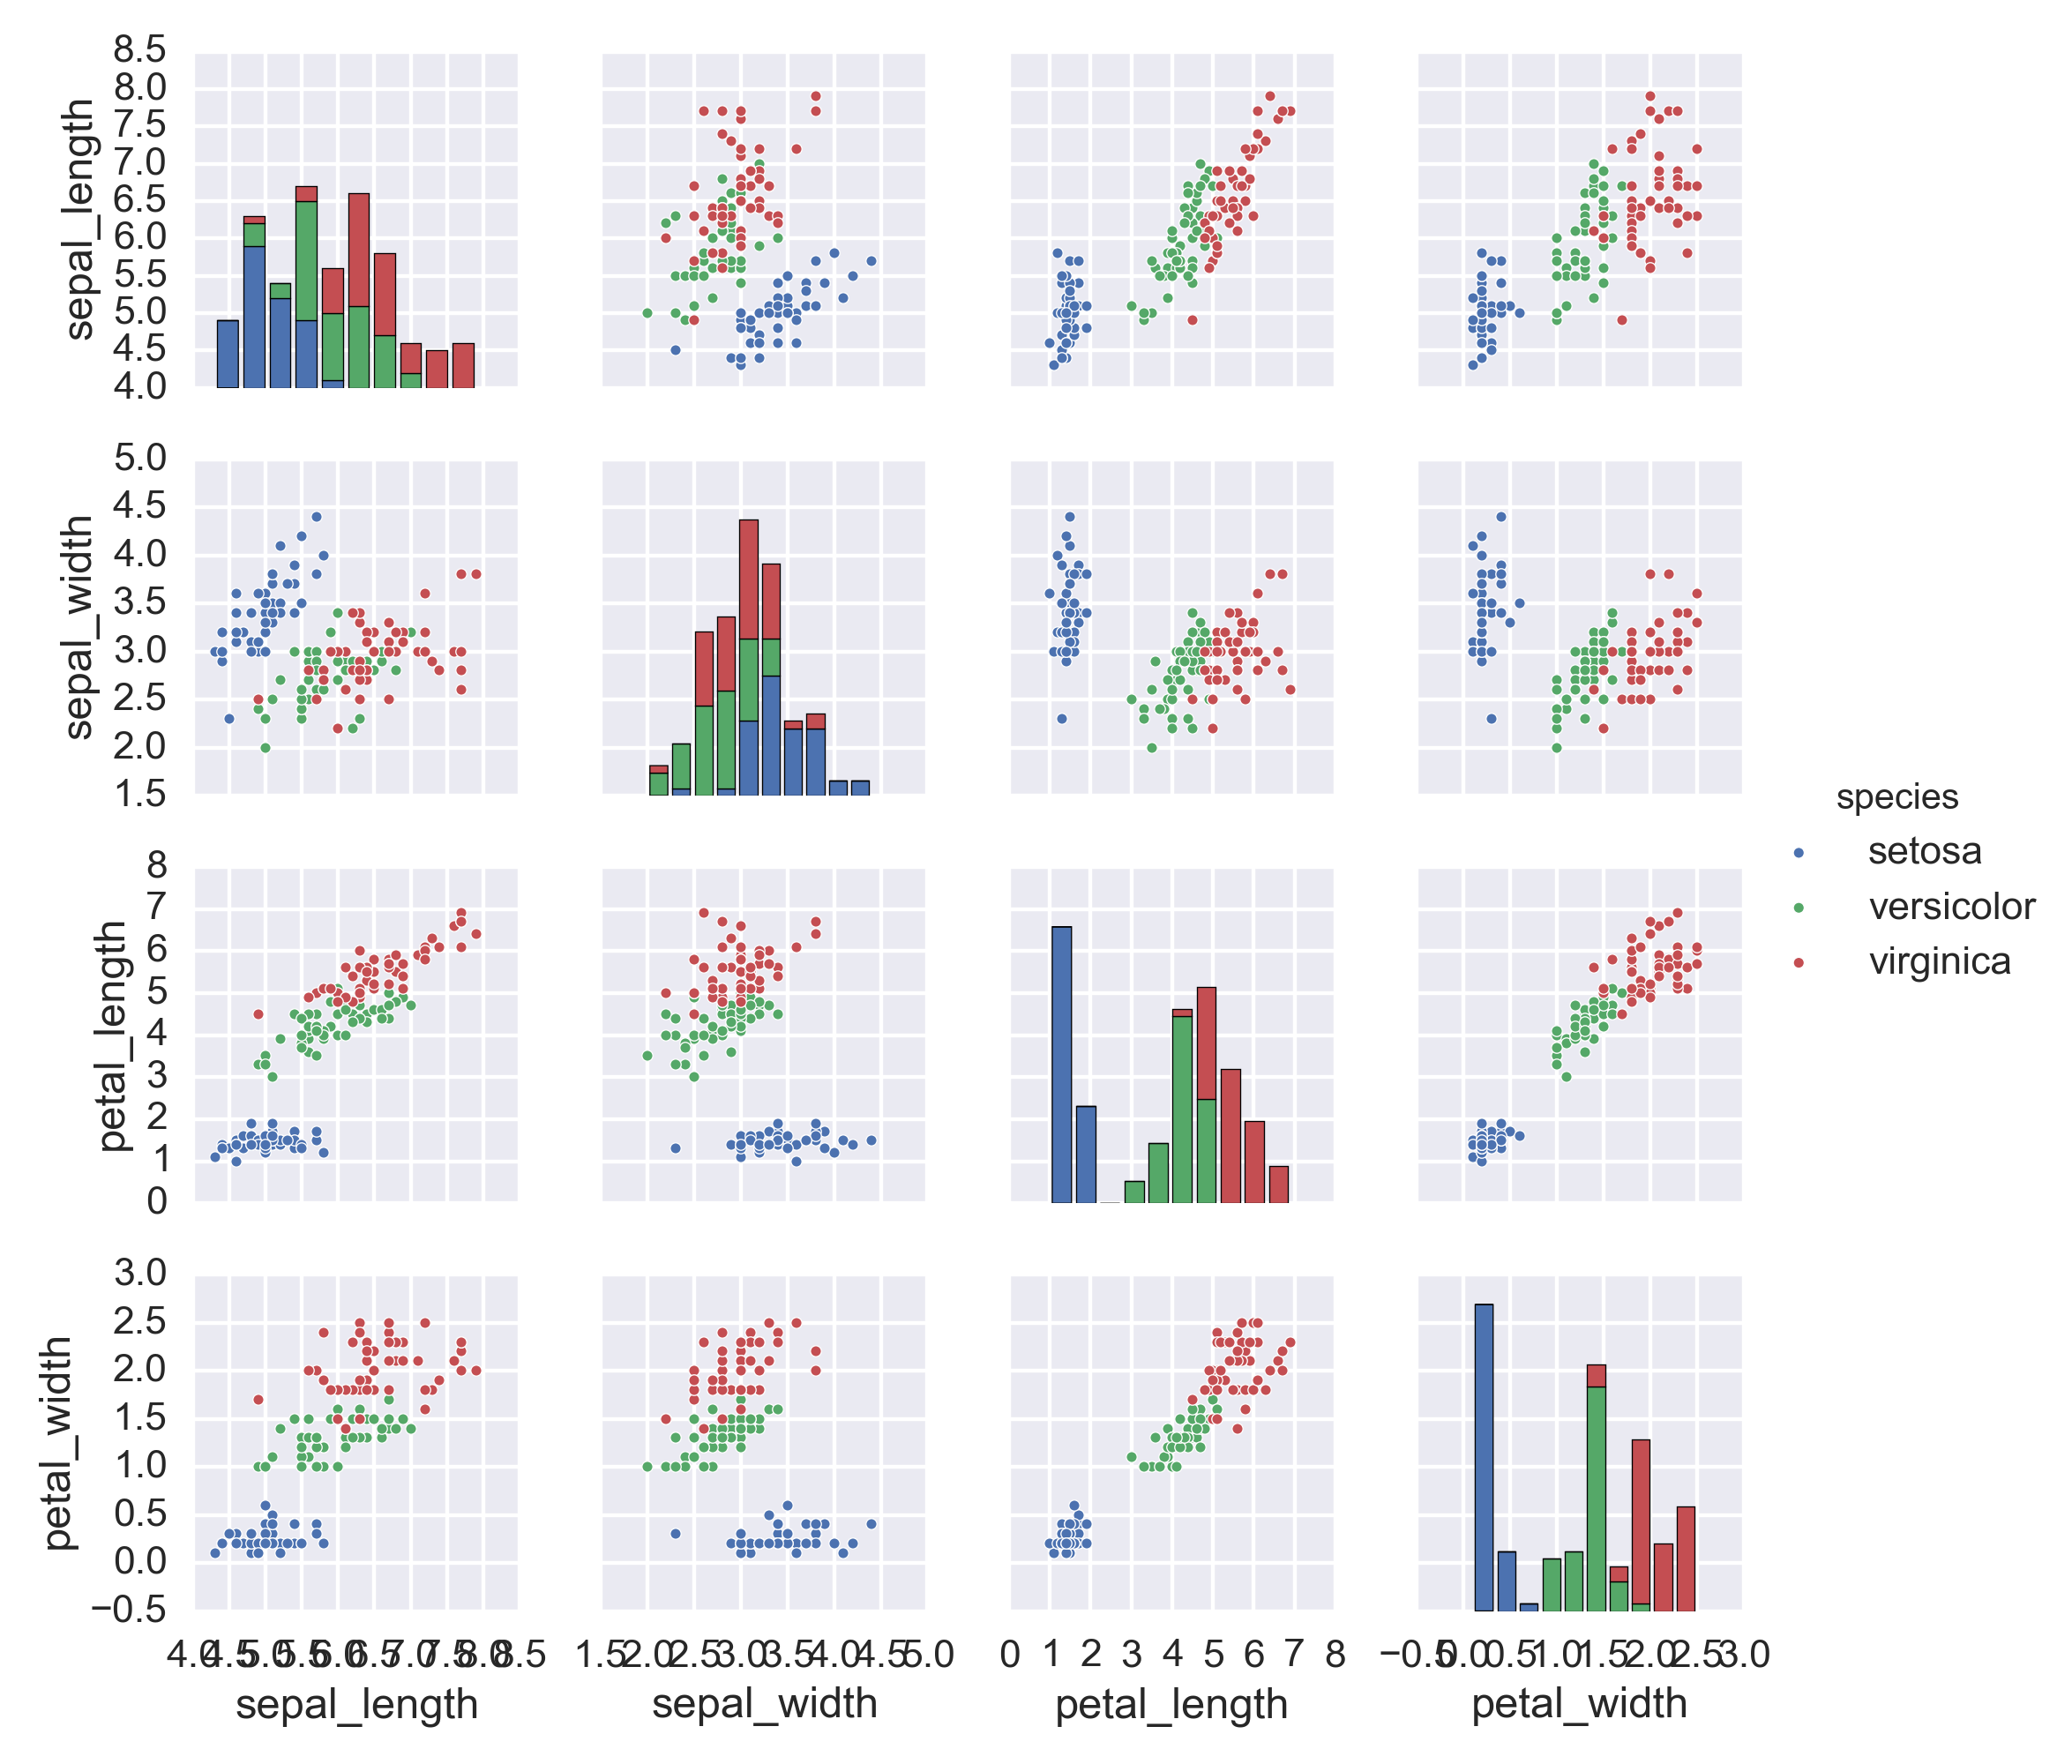
\includegraphics[width=0.85\textwidth]{../Images/multiScatterplot.png}\\
  \caption{Scatterplot matrix.}\label{fig:scatterplotMatrix}
\end{figure}


\subsection{Correlation Matrix}\index{general}{Correlation matrix}

An elegant way to visualize the correlation between a large number of variables is the \emph{correlation matrix}. Using \emph{seaborn}, the following example shows how to implement a correlation matrix. In the example, the parameter for \lstinline{np.random.RandomState} is the seed for the random number generation. The data are normally distributed dummy data, simulating 100 recordings from 30 different variables. The command \lstinline{sns.corrplot} calculates and visualized the cross correlation betwean each possible combination of variables (Fig. \ref:{fig:CorrelationMatrix}):

\begin{figure}
  \centering
  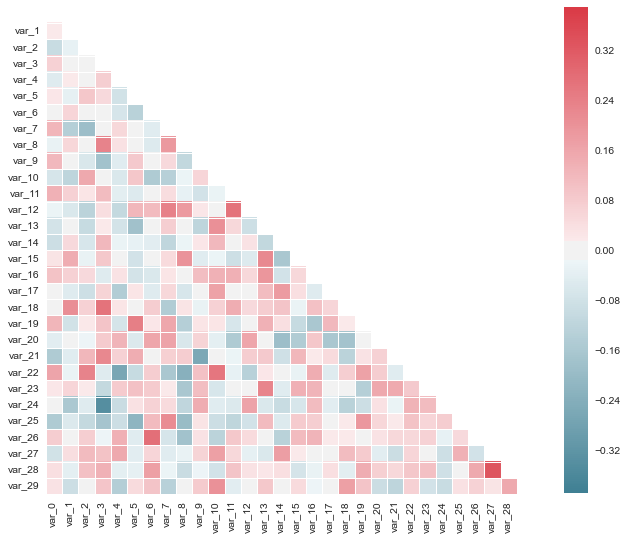
\includegraphics[width=0.75\textwidth]{../Images/many_pairwise_correlations.png}\\
  \caption{Visualization of the Correlation matrix.}\label{fig:CorrelationMatrix}
\end{figure}

\begin{lstlisting}
    import numpy as np
    import seaborn as sns
    import matplotlib.pyplot as plt
    sns.set(style="darkgrid")

    rs = np.random.RandomState(33)
    d = rs.normal(size=(100, 30))

    f, ax = plt.subplots(figsize=(9, 9))
    cmap = sns.diverging_palette(220, 10, as_cmap=True)
    sns.corrplot(d, annot=False, sig_stars=False,
                 diag_names=False, cmap=cmap, ax=ax)
    f.tight_layout()
\end{lstlisting}


\section{Multilinear Regression} \index{general}{regression!multilinear}

If you have truly independent variables, \emph{multilinear regression} is a straightforward extension of the simple linear regression.

\paragraph{Multiple Regression} \index{general}{regression!multiple}
Example of \emph{multiple regression} with covariates (i.e. independent variables) $w_i$ and $x_i$.
Suppose that the data are 7 observations, and for each observed value to be predicted ($y_i$) there are two covariates that were also observed, $w_i$ and $x_i$. The model to be considered is

\begin{equation}
  y_i = \beta_0 + \beta_1 w_i + \beta_2 x_i + \epsilon_i
\end{equation}

This model can be written in matrix terms as

\begin{equation}\label{eq:multipleRegression}
  \begin{bmatrix}y_1 \\ y_2 \\ y_3 \\ y_4 \\ y_5 \\ y_6 \\ y_7 \end{bmatrix} =
    \begin{bmatrix} 1 & w_1 & x_1  \\1 & w_2 & x_2  \\1 & w_3 & x_3  \\1 & w_4 & x_4  \\1 & w_5 & x_5  \\1 & w_6 & x_6 \\ 1& w_7  & x_7  \end{bmatrix}
    \begin{bmatrix} \beta_0 \\ \beta_1 \\ \beta_2  \end{bmatrix}
    +
    \begin{bmatrix} \epsilon_1 \\ \epsilon_2 \\ \epsilon_3 \\ \epsilon_4 \\ \epsilon_5 \\ \epsilon_6 \\ \epsilon_7 \end{bmatrix}
\end{equation}


However, you have to watch out: if your variables may be related to each other, you have to proceed much more carefully. For example, you may want to investigate how the prevalence of some disease correlates with age and with income: if you do so, you have to keep in mind that age and income are most likely correlated! For details, \cite{Kaplan2009} gives a good introduction to that topic. Also, check out the chapter on Modeling.

\PyImg "multipleRegression.py" (p \pageref{py:multipleRegression}): Multiple regression example.
\index{python}{multipleRegression} 